\chapter{Kerutan Otot dan Fungsi Motorik}\label{ch:b2:muscle-movement}

Seorang pelari cepat meninggalkan balok startnya dengan gaya pada
lintasannya sebesar tiga kali beratnya, yang dibangkitkan dalam
seperlima detik oleh otot yang kendur sesaat sebelumnya. Tidak ada apa
pun di dalam selnya yang memendek untuk mengerjakannya: filamen di
dalamnya meluncur saling melewati, ditarik jutaan tangan molekul yang
masing-masing mengambil selangkah sepuluh nanometer lalu melepaskannya,
sepuluh kali tiap detik, yang dibayar satu ATP tiap kalinya. Bab ini
mengambil \omterm{def:b2:cell-differentiation:myogenesis}{serabut otot} yang dibangun pada
\cref{ch:b2:cell-differentiation} lalu membuatnya bekerja: peluncuran
filamennya dan motor yang menggerakkannya, sakelar kalsium yang
menyalakan dan memadamkan motornya, perintah dari sarafnya, mekanika
gaya dan kecepatannya, serta cara sistem sarafnya menjenjangkan
keseluruhannya dari sebuah \omterm{def:b2:muscle-movement:motorunit}{kedutan} sampai sebuah lari cepat.

\section{Filamen yang meluncur}

\begin{proposition}[Mekanisme filamen luncur]\label{prop:b2:muscle-movement:sliding}
\index{filamen luncur}\index{sarkomer!kerutan}
Ketika sebuah \omterm{def:b2:cell-differentiation:myogenesis}{serabut otot} memendek, \omterm{def:b2:cell-differentiation:fibre}{sarkomernya} memendek
(\cref{ch:b2:cell-differentiation}), tetapi baik filamen tebal miosin
maupun filamen tipis aktin tidak berubah panjangnya: filamen tipisnya
meluncur ke dalam sepanjang filamen tebalnya, pita I dan zona H-nya
menyempit, dan cakram Z-nya saling mendekat. Tindihan antara kedua
perangkat filamennya adalah tempat gayanya dibangkitkan, dan sebuah
\omterm{def:b2:cell-differentiation:fibre}{sarkomer} membangkitkan gaya sebanding dengan tindihannya: dari panjang
teregang \qty{3.6}{\micro m}, yang tanpa tindihan dan tanpa gaya,
gayanya naik secara lurus ketika filamennya bertindih lebih banyak,
mencapai sebuah dataran mendekati \qty{2.2}{\micro m} yang padanya tiap
kepala miosin menghadap aktin, lalu turun lagi di bawah
\qty{2.0}{\micro m} ketika filamen tipisnya bertumbukan dan filamen
tebalnya membentur cakram Z-nya. Panjang istirahat sebuah otot di dalam
tubuhnya berada pada datarannya --- dan itulah petunjuk pertama tentang
bagaimana gayanya dibuat.
\end{proposition}
\begin{proof}[Bukti eksperimental]
A.~F.~Huxley dan Niedergerke, serta H.~E.~Huxley dan Hanson (1954),
mengukur pita serabut tunggal dan \omterm{def:b2:cell-differentiation:fibre}{miofibril} terpencil dengan mikroskopi
interferensi dan fase ketika serabutnya memendek: pita A-nya menjaga
panjangnya, pita I-nya menyusut, sehingga filamennya meluncur. Gordon,
Huxley, dan Julian (1966) menahan sebuah serabut tunggal pada panjang
yang ditetapkan dengan sebuah alat umpan balik yang menjaga \omterm{def:b2:cell-differentiation:fibre}{sarkomer}
satu ruasnya tetap panjangnya, lalu menemukan bahwa gayanya sebanding
dengan tindihan filamen tebal dan tipisnya yang diukur dengan mikroskopi
elektron --- yaitu kurva panjang--tegangan beserta datarannya dan kedua
tungkai lurusnya, tepat seperti yang diramalkan geometri filamennya.
\end{proof}

\begin{omfigure}
\begin{minipage}[b]{0.5\linewidth}\centering
\begin{tikzpicture}[every node/.style={font=\scriptsize}]
  \foreach \y/\lab/\ov in {2.4/{mengendur, \qty{2.6}{\micro m}}/0.9, 1.2/{berkerut, \qty{2.0}{\micro m}}/0.3} {
    \begin{scope}[yshift=\y cm]
      \draw[very thick, omThm] (0,-0.35) -- (0,0.35); \draw[very thick, omThm] (4.4-2*\ov+1.0,-0.35) -- (4.4-2*\ov+1.0,0.35);
      \pgfmathsetmacro{\len}{4.4-2*\ov+1.0}
      \foreach \dy in {-0.25,0.05,0.25} { \draw[thick, omDef] (0,\dy) -- (1.5,\dy); \draw[thick, omDef] (\len,\dy) -- (\len-1.5,\dy); }
      \draw[line width=3pt, omExo!80!black] (\len/2-1.1,-0.1) -- (\len/2+1.1,-0.1);
      \node[right] at (\len+0.15,0) {\lab};
    \end{scope}
  }
  \node[align=center] at (2.7,0.1) {filamennya menjaga panjangnya;\\tindihannya bertambah ketika cakram Z mendekat};
\end{tikzpicture}
\end{minipage}\hfill
\begin{minipage}[b]{0.48\linewidth}\centering
\begin{tikzpicture}
\begin{axis}[
  width=\linewidth, height=4.8cm,
  axis x line=bottom, axis y line=left,
  xmin=1.2, xmax=3.8, ymin=0, ymax=1.15,
  xlabel={panjang sarkomer (\unit{\micro m})}, ylabel={gaya (nisbi)},
  xlabel style={font=\scriptsize, at={(axis description cs:0.5,-0.17)}, anchor=north},
  ylabel style={font=\scriptsize},
  tick label style={font=\scriptsize}, xtick={1.3,2.0,2.2,3.6}, ytick={0,0.5,1},
  clip=false,
]
\addplot[very thick, omDef] coordinates {(1.3,0) (1.65,0.5) (2.0,1) (2.2,1) (3.6,0)};
\node[font=\scriptsize, anchor=south] at (axis cs:2.1,1.02) {dataran};
\node[font=\scriptsize, anchor=west, align=left] at (axis cs:2.95,0.75) {tindihannya\\berkurang};
\end{axis}
\end{tikzpicture}
\end{minipage}

{\small Kiri: sebuah \omterm{def:b2:cell-differentiation:fibre}{sarkomer} yang mengendur dan yang berkerut ---
filamen tipisnya (biru) meluncur sepanjang filamen tebalnya (kelabu)
tanpa berubah panjangnya. Kanan: kurva panjang--tegangannya: gayanya
sebanding dengan tindihannya, dan maksimal pada datarannya tempat
ototnya beristirahat.}
\end{omfigure}

\begin{omfigure}
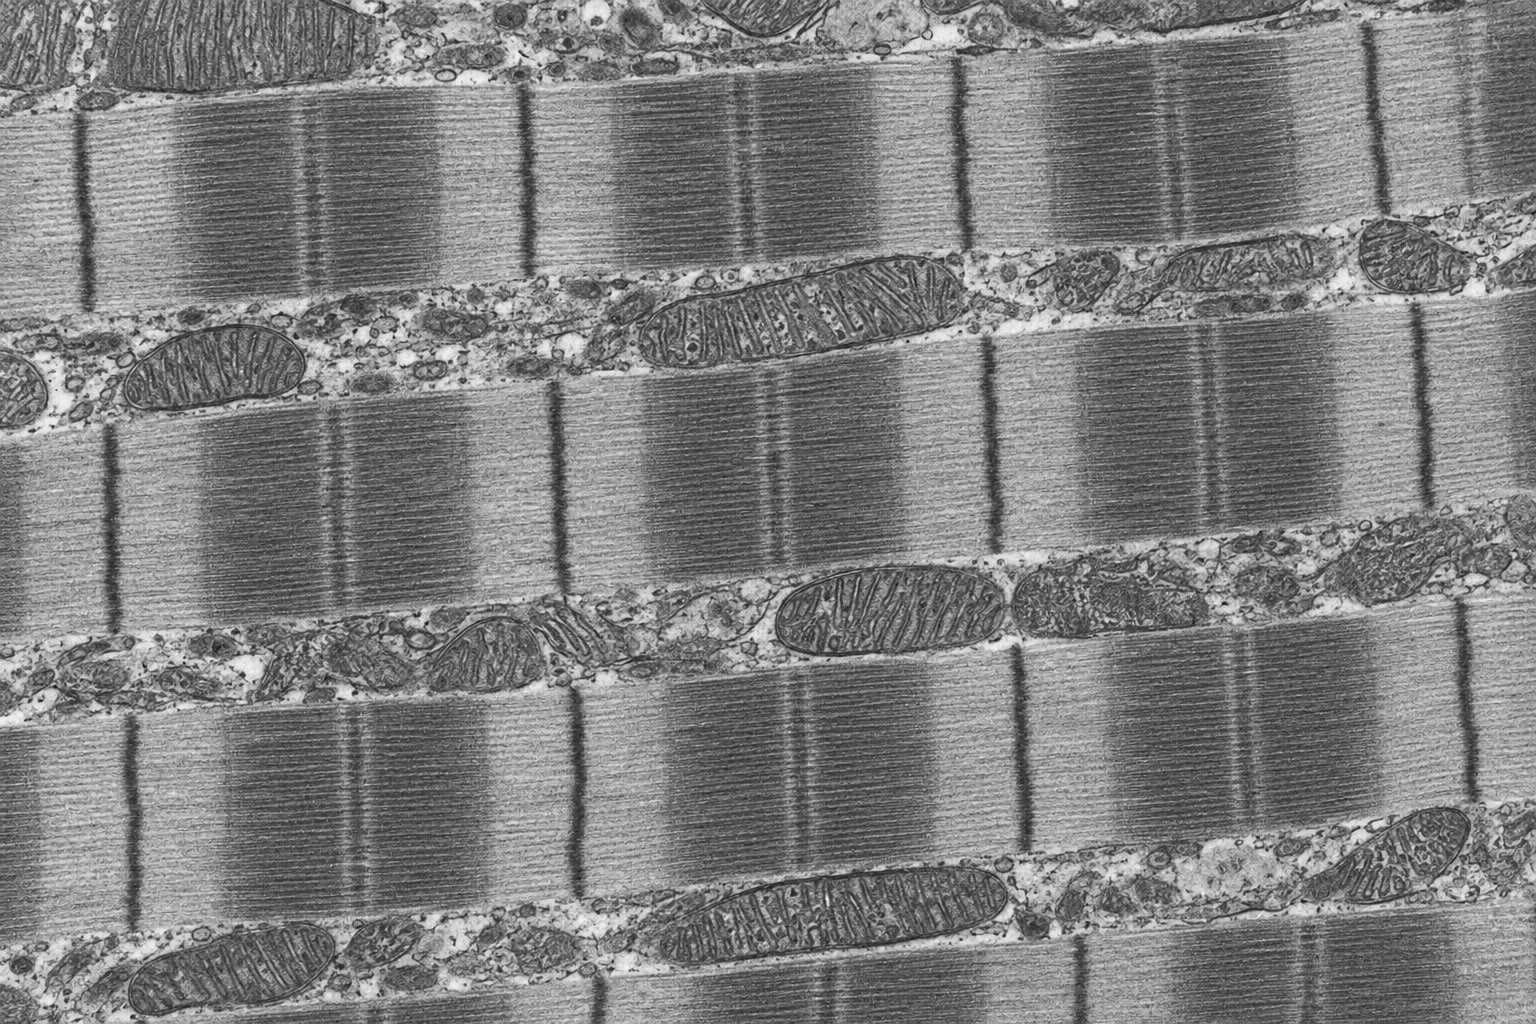
\includegraphics[width=0.6\linewidth]{images/book4/ai/b4-21-sarcomere-tem.jpg}

{\small \omterm{def:b2:cell-differentiation:fibre}{Miofibril} di bawah mikroskop elektron: pita A filamen tebalnya,
pita I filamen tipisnya yang dibelah dua garis Z, dan mitokondria di
antara fibrilnya yang membayar peluncurannya.}
\end{omfigure}

\section{Motornya}

\begin{proposition}[Daur jembatan silang]\label{prop:b2:muscle-movement:crossbridge}
\index{daur jembatan silang}\index{miosin}\index{ATP!pada kerutan}
Tiap filamen tebal berbulu kira-kira tiga ratus \emph{kepala miosin},
dan tiap kepalanya adalah sebuah motor yang berjalan sepanjang aktin
dalam sebuah daur berlangkah empat. (1) Dengan ATP yang terikat,
kepalanya terlepas dari aktinnya; ia menghidrolisis ATP-nya menjadi ADP
dan fosfat lalu menegangkan dirinya menjadi sebuah bentuk yang terikat
tegangan dan berenergi tinggi. (2) Kepala yang tertegang itu mengikat
sebuah subunit aktin, sehingga membentuk sebuah \emph{jembatan silang}.
(3) Fosfatnya dilepaskan dan kepalanya menyentak ke bentuknya yang
kendur, sambil menarik filamen tipisnya kira-kira \qty{10}{nm} menuju
pusat \omterm{def:b2:cell-differentiation:fibre}{sarkomernya} --- yaitu \emph{langkah tenaganya}; ADP-nya pergi.
(4) Sebuah ATP yang baru mengikat dan kepalanya melepaskan aktinnya;
tanpa ATP ia tidak dapat melepaskannya, dan itulah kekakuan kematian.
Daurnya memakan waktu kira-kira seperdua puluh detik; sebuah kepala
menghabiskan sebagian besar waktunya dalam keadaan terlepas, sehingga
pada tiap saatnya hanya sebagian kepalanya yang menarik, dan sebuah
filamen yang meluncur cepat tidak pernah terjatuh. Gayanya adalah jumlah
tarikan kepala yang terikat; pemendekannya adalah jumlah langkahnya,
paling banyak setengah mikrometer tiap \omterm{def:b2:cell-differentiation:fibre}{sarkomer} tiap daurnya; dan
energinya adalah satu ATP tiap langkah tiap kepalanya, kira-kira
\qty{50}{kJ/mol} --- \qty{8e-20}{J} tiap langkah, yang sampai
separuhnya diubah kepalanya menjadi kerja.
\end{proposition}

\begin{omfigure}
\begin{tikzpicture}[every node/.style={font=\scriptsize}, >=stealth]
  \foreach \x/\lab/\ang/\att in {0/{1. ATP terikat:\\terlepas; ATP\\terhidrolisis, kepala tertegang}/60/0, 3.6/{2. kepala tertegang\\mengikat aktin:\\jembatan silang}/60/1, 7.2/{3. fosfat dilepaskan:\\langkah tenaga,\\filamen ditarik \qty{10}{nm}}/20/1, 10.8/{4. ADP pergi, ATP\\baru mengikat: kepala\\melepaskannya}/20/0} {
    \begin{scope}[xshift=\x cm]
      \draw[thick, omDef] (0,2.2) -- (2.8,2.2); \foreach \i in {0.2,0.6,...,2.6} \fill[omDef!50] (\i,2.2) circle (0.14);
      \draw[line width=3pt, omExo!80!black] (0,0.4) -- (2.8,0.4);
      \draw[very thick, omThm] (1.4,0.4) -- (1.4,1.0);
      \ifnum\att=1 \draw[very thick, omThm] (1.4,1.0) -- ++(\ang:1.15); \fill[omThm] (1.4,1.0) ++(\ang:1.15) circle (0.16); \else \draw[very thick, omThm] (1.4,1.0) -- ++(\ang:1.0); \fill[omThm] (1.4,1.0) ++(\ang:1.0) circle (0.16); \fi
      \node[below, align=center] at (1.4,0.15) {\lab};
    \end{scope}
  }
  \draw[->, thick, omDef] (7.9,2.55) -- (8.9,2.55); \node[omDef, above] at (8.4,2.6) {filamen tipisnya bergerak};
\end{tikzpicture}

{\small \omterm{prop:b2:muscle-movement:crossbridge}{Daur jembatan silangnya}. Sebuah kepala miosin yang tertegang
(merah) mengikat aktin (biru), melepaskan fosfat lalu menarik filamen
tipisnya lewat langkah tenaganya, kemudian mengikat sebuah ATP yang
segar lalu melepaskannya.}
\end{omfigure}

\begin{theorem}[Gaya, kecepatan, dan daya sebuah otot]\label{thm:b2:muscle-movement:hill}
\index{kurva gaya--kecepatan}\index{daya otot}
Gaya sebuah otot turun ketika ia memendek lebih cepat, karena makin
cepat filamennya meluncur, makin sedikit kepala yang terikat pada tiap
saatnya dan makin banyak kepala yang terseret melewati langkahnya
sebelum ia melepaskannya. Hubungan Hill memerikannya:
\[
(F + a)(v + b) = (F_0 + a)\,b,
\]
dengan $F_0$ adalah gaya isometriknya (pada $v = 0$), $v_{\max} =
F_0 b/a$ adalah kecepatan tanpa bebannya, dan $a$, $b$ adalah tetapan
($a \approx
F_0/4$). Dayanya $Fv$ bernilai nol pada kedua ujungnya dan
terbesar pada kira-kira sepertiga $v_{\max}$ dan sepertiga $F_0$ ---
itulah sebabnya seorang pesepeda mengganti giginya dan langkah seorang
pelari cepat memiliki laju yang disukainya. Sebuah otot manusia
membangkitkan kira-kira \qty{30}{N} tiap sentimeter persegi
penampangnya, memendek sampai sepuluh panjangnya tiap detik, dan
mengantarkan sekitar \qty{100}{W} tiap kilogram pada keadaan terbaiknya.
\end{theorem}
\begin{proof}
Kurva Hill bersifat empiris (1938), yang diukur pada otot katak yang
terpencil sebagai kecepatan pemendekannya terhadap beban yang ia
angkat; hiperbolanya cocok karena bagian kepala yang terikat turun
bersama kecepatan luncurnya dan gaya tiap kepala yang terikat turun
ketika ia terbawa melewati langkahnya. Dayanya: dengan $F = (F_0 + a)b/(v + b) - a$, $Fv$ bernilai nol pada $v = 0$ dan pada $v_{\max}$;
mendiferensialkannya memberikan maksimumnya pada
$v = b(\sqrt{(F_0 + a)/a} - 1)$, yang bagi $a = F_0/4$ adalah $v =
1.24\,b = 0.31\,v_{\max}$, yang padanya $F = 0.31\,F_0$.
\end{proof}

\begin{omfigure}
\begin{tikzpicture}
\begin{axis}[
  width=0.7\linewidth, height=5.4cm,
  axis x line=bottom, axis y line=left,
  xmin=0, xmax=1.05, ymin=0, ymax=1.1,
  xlabel={kecepatan pemendekan $v/v_{\max}$}, ylabel={gaya $F/F_0$, daya (nisbi)},
  xlabel style={font=\small, at={(axis description cs:0.5,-0.13)}, anchor=north},
  ylabel style={font=\small},
  tick label style={font=\small}, xtick={0,0.31,1}, xticklabels={0,0.31,1}, ytick={0,0.31,1}, yticklabels={0,0.31,1},
  legend style={font=\scriptsize, at={(0.97,0.95)}, anchor=north east, draw=none},
  clip=false,
]
\addplot[very thick, omDef, domain=0:1, samples=100] {(1.25*0.25)/(x+0.25) - 0.25};
\addlegendentry{gaya}
\addplot[very thick, omThm, domain=0:1, samples=100] {10.4*x*((1.25*0.25)/(x+0.25) - 0.25)};
\addlegendentry{daya (terskalakan)}
\draw[dashed, gray] (axis cs:0.31,0) -- (axis cs:0.31,1.0);
\end{axis}
\end{tikzpicture}

{\small \omterm{thm:b2:muscle-movement:hill}{Kurva gaya--kecepatan} Hill ($a = F_0/4$) dan daya yang
disiratkannya: gayanya turun ketika ototnya memendek lebih cepat, dan
dayanya memuncak pada kira-kira sepertiga kecepatan maksimalnya dan
sepertiga gaya isometriknya.}
\end{omfigure}

\section{Sakelarnya: kalsium}

\begin{proposition}[Penggandengan rangsang--kerut]\label{prop:b2:muscle-movement:coupling}
\index{penggandengan rangsang--kerut}\index{troponin}\index{tropomiosin}\index{retikulum sarkoplasma}
Ketika beristirahat kepala miosinnya tidak dapat mencapai aktinnya:
tapak pengikat pada filamen tipisnya tertutup oleh \emph{tropomiosin},
sebatang tongkat yang terbaring di dalam alur heliks aktinnya, yang
ditahan di sana oleh \emph{troponin}. Sakelarnya adalah kalsium. Sebuah
\omterm{prop:b2:neurons-synapses:ap}{potensial aksi} pada membran serabutnya berjalan turun lewat \omterm{def:b2:cell-differentiation:fibre}{tubulus
T-nya} menuju bagian dalamnya lalu, pada persambungan tempat sebuah
\omterm{def:b2:cell-differentiation:fibre}{tubulus T} berjumpa dengan \omterm{def:b2:cell-differentiation:fibre}{retikulum sarkoplasmanya}, membuka kanal
pelepas kalsium retikulumnya; kalsiumnya membanjiri \omterm{def:b2:cell-differentiation:fibre}{miofibrilnya}, naik
dari \qty{0.1}{} menjadi \qty{10}{\micro mol/L} dalam semilidetik,
mengikat troponinnya, dan troponinnya menggeser tropomiosinnya menjauhi
tapak pengikatnya: kepalanya melekat, dan serabutnya berkerut selama
kalsiumnya tetap ada. Pompa di dalam retikulumnya, yang membakar ATP,
mengambil kalsiumnya kembali dalam puluhan milidetik; tropomiosinnya
menutupi kembali tapaknya dan serabutnya mengendur. Karena itu
pengenduran sama aktifnya dengan kerutan, dan sebuah otot yang
kekurangan ATP tidak dapat melepaskan kepalanya maupun memompa
kalsiumnya --- rigor mortis. Di dalam \omterm{def:b2:heart:anatomy}{jantungnya} sakelar yang sama
dipakai, tetapi dengan kalsium yang masuk dari luar lewat kanal
membrannya sendiri untuk memicu pelepasannya, dan itulah sebabnya
\omterm{def:b2:heart:anatomy}{jantungnya}, dan bukan otot rangkanya, peka terhadap kalsium di dalam
\omterm{def:b2:blood-circulation:blood}{darahnya}.
\end{proposition}

\begin{omfigure}
\begin{tikzpicture}[every node/.style={font=\scriptsize}, >=stealth]
  \node[draw, rounded corners, fill=omDef!15, align=center] (nerve) at (0,0) {impuls saraf\\motorik};
  \node[draw, rounded corners, fill=omDef!15, align=center] (nmj) at (3.0,0) {sambungan\\saraf-otot:\\asetilkolin};
  \node[draw, rounded corners, fill=omDef!15, align=center] (ap) at (6.2,0) {potensial aksi otot,\\turun lewat\\tubulus T};
  \node[draw, rounded corners, fill=omThm!15, align=center] (ca) at (9.4,0) {Ca$^{2+}$ dilepaskan\\dari retikulum\\sarkoplasmanya};
  \node[draw, rounded corners, fill=omProp!20, align=center] (tn) at (12.6,0) {troponin mengikat Ca$^{2+}$,\\tropomiosin bergeser,\\kepalanya melekat};
  \node[draw, rounded corners, fill=omExo!25, align=center] (off) at (9.4,-2.2) {pompa mengembalikan Ca$^{2+}$ (ATP);\\tropomiosin menutupi aktin lagi:\\pengenduran};
  \draw[->, thick] (nerve) -- (nmj); \draw[->, thick] (nmj) -- (ap); \draw[->, thick] (ap) -- (ca); \draw[->, thick] (ca) -- (tn);
  \draw[->, thick] (ca) -- (off);
  \node[below, gray] at (1.5,-0.7) {\qty{0.6}{ms}}; \node[below, gray] at (4.6,-0.7) {\qty{1}{ms}}; \node[below, gray] at (7.8,-0.7) {\qty{1}{ms}};
\end{tikzpicture}

{\small Dari impuls saraf sampai gaya: persambungannya, \omterm{prop:b2:neurons-synapses:ap}{potensial aksi}
serabutnya sendiri, pelepasan kalsiumnya, dan penyingkapan tapak
aktinnya --- lalu pompa yang mengakhirinya.}
\end{omfigure}

\section{Perintah dan penjenjangan}

\begin{definition}[Unit motorik]\label{def:b2:muscle-movement:motorunit}
\index{unit motorik}\index{kedutan}\index{tetanus}\index{perekrutan}
Sebuah \emph{\omterm{def:b2:neurons-synapses:neuron}{neuron} motorik} di dalam sumsum tulang belakangnya
mengirimkan \omterm{def:b2:neurons-synapses:neuron}{aksonnya} ke sebuah otot lalu bercabang untuk menyarafi dari
segelintir sampai seribu serabut, yang bertaburan di seluruh ototnya;
\omterm{def:b2:neurons-synapses:neuron}{neuronnya} beserta serabutnya adalah sebuah \emph{unit motorik}, yaitu
kuantitas gaya terkecil yang dapat diperintahkan sistem sarafnya. Tiap
impuls di dalam \omterm{def:b2:neurons-synapses:neuron}{neuronnya} membuat tiap serabut unitnya memicu sekali
lalu memberikan sebuah \emph{kedutan}: sebuah gaya yang naik dalam
kira-kira \qty{30}{ms} lalu meluruh dalam \qty{100}{ms}, karena denyut
kalsiumnya singkat. Impuls yang berturut-turut dengan cepat membuat
kedutannya berjumlah, karena kalsium dari yang satu belum terpompa
pergi ketika yang berikutnya tiba; pada kira-kira 30 sampai 50 impuls
tiap detik gayanya melebur menjadi sebuah \emph{tetanus} yang mulus,
yaitu tiga sampai lima kali kedutannya. Sistem sarafnya menjenjangkan
gaya sebuah otot dengan dua cara: dengan \emph{laju} tiap unitnya
memicu, dan dengan \emph{jumlah} unit yang ia rekrut --- unit yang
kecil, lambat, dan tahan lelah lebih dahulu (yaitu \emph{asas
ukuran}), unit yang besar dan cepat terakhir, hanya bagi usaha yang
terbesar. Karena itu sebuah otot dalam pemakaian biasa tidak pernah
menyala penuh: sebagian unitnya memicu, secara bergiliran, dan sisanya
beristirahat.
\end{definition}

\begin{omfigure}
\begin{tikzpicture}
\begin{axis}[
  width=0.82\linewidth, height=5.4cm,
  axis x line=bottom, axis y line=left,
  xmin=0, xmax=1.0, ymin=0, ymax=4.2,
  xlabel={waktu (s)}, ylabel={gaya (kedutan $=$ 1)},
  xlabel style={font=\small, at={(axis description cs:0.5,-0.13)}, anchor=north},
  ylabel style={font=\small},
  tick label style={font=\small}, xtick={0,0.2,0.4,0.6,0.8,1}, ytick={0,1,2,3,4},
  clip=false,
]
% single twitch
\addplot[very thick, omDef, domain=0:0.2, samples=60] {(x<0.02)*0 + (x>=0.02)*4.5*(x-0.02)*exp(-(x-0.02)/0.03)*4.1};
% summation at 10 Hz
\addplot[very thick, omProp, domain=0.25:0.62, samples=200] {(x>=0.25)*4.5*4.1*(x-0.25)*exp(-(x-0.25)/0.03) + (x>=0.33)*4.5*4.1*(x-0.33)*exp(-(x-0.33)/0.03) + (x>=0.41)*4.5*4.1*(x-0.41)*exp(-(x-0.41)/0.03) + (x>=0.49)*4.5*4.1*(x-0.49)*exp(-(x-0.49)/0.03)};
% tetanus at 50 Hz
\addplot[very thick, omThm, domain=0.66:0.98, samples=100] {3.8*(1-exp(-(x-0.66)/0.06))};
\node[font=\scriptsize, anchor=west] at (axis cs:0.09,0.7) {satu impuls: kedutan};
\node[font=\scriptsize, anchor=south] at (axis cs:0.44,2.2) {\qty{12}{Hz}: penjumlahan};
\node[font=\scriptsize, anchor=south] at (axis cs:0.82,3.85) {\qty{50}{Hz}: tetanus yang melebur};
\end{axis}
\end{tikzpicture}

{\small Menjenjangkan gaya dengan laju. Sebuah impuls tunggal
memberikan sebuah \omterm{def:b2:muscle-movement:motorunit}{kedutan}; impuls pada selusin tiap detik berjumlah
menjadi sebuah gaya yang beriak; pada lima puluh tiap detik gayanya
melebur menjadi sebuah \omterm{def:b2:muscle-movement:motorunit}{tetanus} yang beberapa kali \omterm{def:b2:muscle-movement:motorunit}{kedutannya}.}
\end{omfigure}

\begin{proposition}[Refleks dan sumsum tulang belakangnya]\label{prop:b2:muscle-movement:reflex}
\index{busur refleks}\index{kumparan otot}\index{refleks regang}\index{penghambatan timbal balik}
\omterm{def:b2:neurons-synapses:neuron}{Neuron} motoriknya adalah \emph{jalur bersama akhirnya}: tiap perintah,
entah dari korteksnya atau dari sebuah refleks, berakhir padanya.
Untaian yang paling sederhana adalah \emph{\omterm{prop:b2:muscle-movement:reflex}{refleks regang}} pada
\cref{ch:b2:neurons-synapses}: ujung sensorik yang terlilit mengelilingi
serabut khusus di dalam ototnya, yaitu \emph{\omterm{prop:b2:muscle-movement:reflex}{kumparan ototnya}}, memicu
ketika ototnya teregang, merangsang \omterm{def:b2:neurons-synapses:neuron}{neuron} motorik otot yang sama lewat
satu \omterm{def:b2:neurons-synapses:synapse}{sinapsis}, lalu menghambat \omterm{def:b2:neurons-synapses:neuron}{neuron} motorik lawannya lewat sebuah
interneuron (\emph{\omterm{prop:b2:muscle-movement:reflex}{penghambatan timbal balik}}), sehingga ototnya
melawan regangannya --- yaitu dasar sikap tubuhnya, karena tiap ayunan
adalah sebuah regangan pada suatu otot. Sebuah reseptor kedua, yaitu
organ tendonnya, memicu ketika gaya ototnya tinggi lalu menghambat
\omterm{def:b2:neurons-synapses:neuron}{neuron} motoriknya sendiri: sebuah katup pengaman. Menarik diri dari
sebuah rangsangan yang menyakitkan adalah sebuah refleks berisi
beberapa \omterm{def:b2:neurons-synapses:synapse}{sinapsis} yang membengkokkan anggota geraknya dan, pada sisi
yang lain, meluruskan anggota gerak yang satunya sehingga Anda tidak
jatuh. Dan otaknya tidak memerintahkan otot melainkan gerakan:
korteksnya mengirimkan sebuah rencana, otak kecilnya membetulkannya
terhadap apa yang dilaporkan kumparannya, ganglia basalnya
melepaskannya, dan untaian sumsum tulang belakangnya, yang dapat
menjalankan sebuah irama melangkah sendiri, melaksanakannya --- yaitu
pokok bahasan jilid Tahun 3.
\end{proposition}

\begin{omfigure}
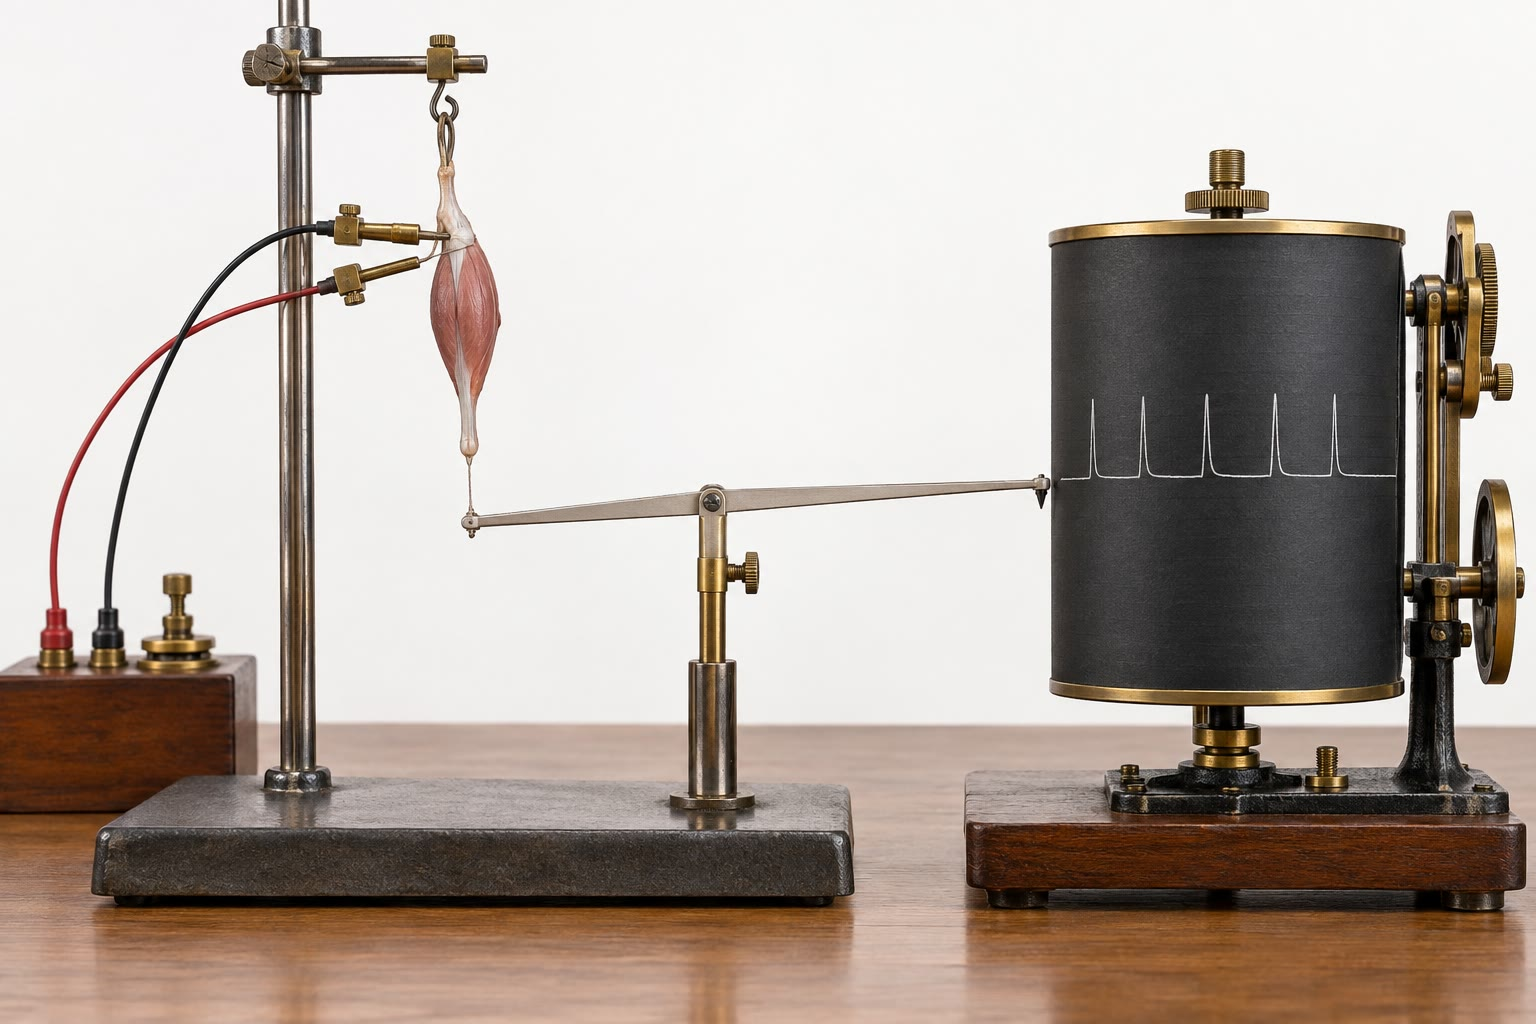
\includegraphics[width=0.44\linewidth]{images/book4/ai/b4-21-frog-muscle-prep.jpg}\hspace{0.04\linewidth}
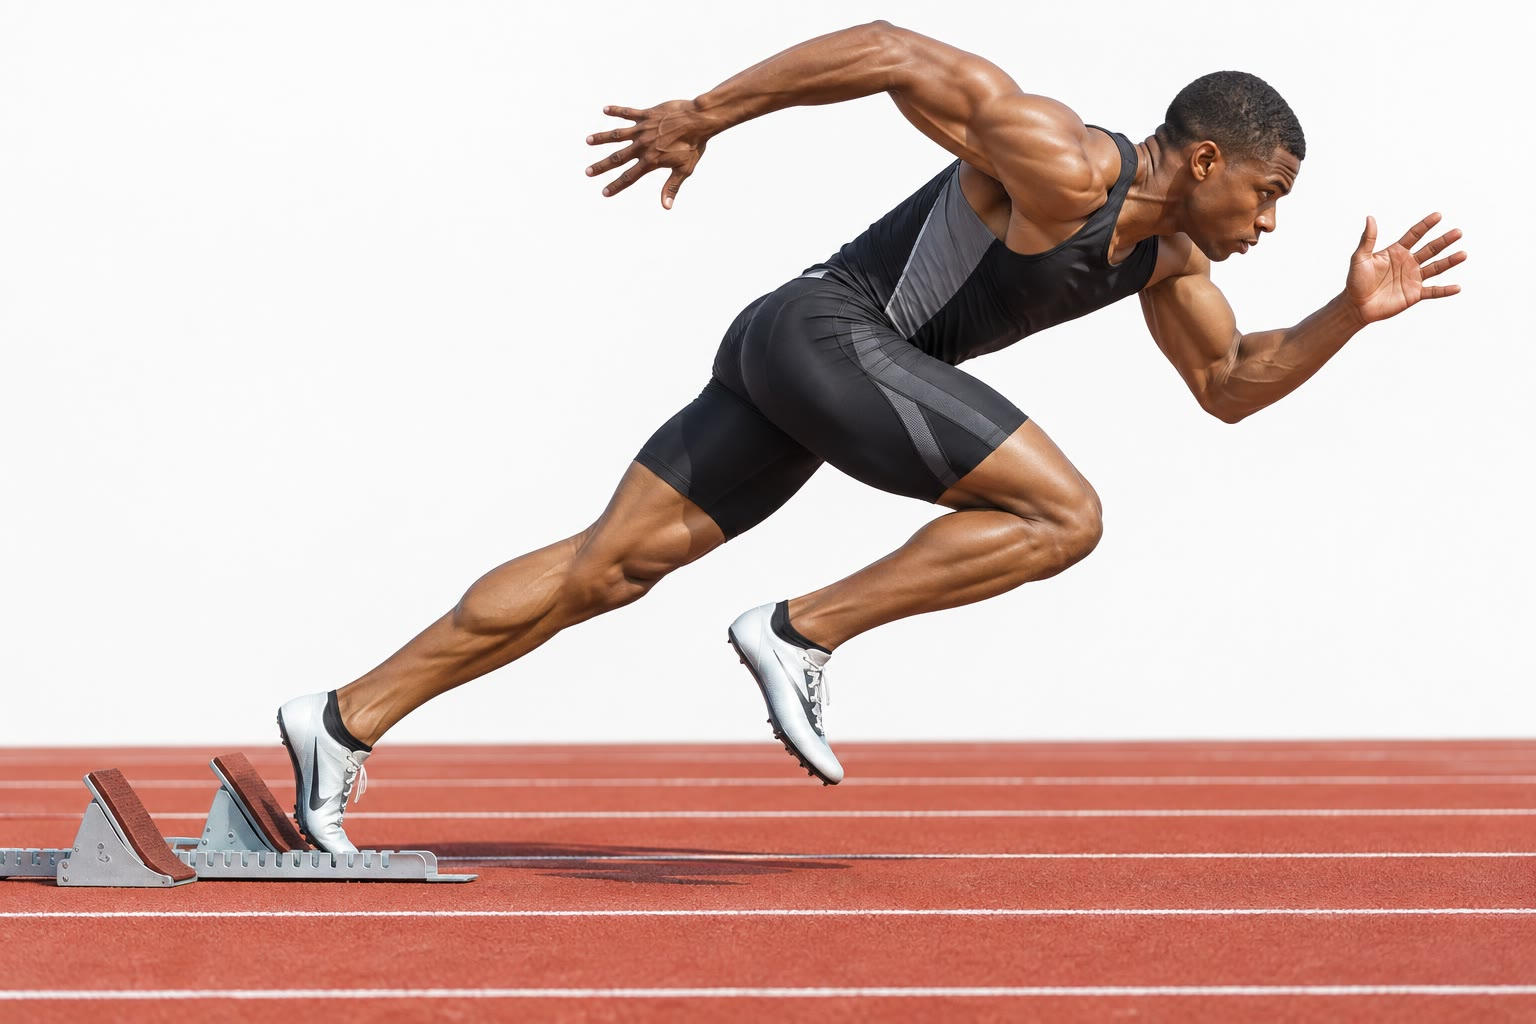
\includegraphics[width=0.44\linewidth]{images/book4/ai/b4-21-sprinter.jpg}

{\small Kiri: sediaan klasiknya --- sebuah otot katak, sarafnya,
elektrode perangsang, dan sebuah tuas yang menulis pada sebuah tromol
berjelaga --- yang padanya \omterm{def:b2:muscle-movement:motorunit}{kedutan}, penjumlahan, dan \omterm{def:b2:muscle-movement:motorunit}{tetanus} pertama
kali direkam. Kanan: faal yang sama pada regangan penuhnya.}
\end{omfigure}

\section{Bahan bakar dan kelelahan}

\begin{proposition}[Membayar kerjanya]\label{prop:b2:muscle-movement:energy}
\index{kreatin fosfat}\index{kelelahan otot}\index{utang oksigen}
Sebuah serabut menahan ATP bagi satu atau dua detik usaha penuh.
Cadangan pertamanya adalah \emph{\omterm{prop:b2:muscle-movement:energy}{kreatin fosfat}}, yang memfosforilasi
ulang ADP dalam hitungan milidetik dan bertahan kira-kira sepuluh detik
--- yaitu bahan bakar pelari cepatnya. Yang kedua adalah
\emph{glikolisis} glikogen serabutnya, tanpa oksigen, yang menghasilkan
dua ATP tiap glukosa beserta laktat: cepat, cukup bagi satu atau dua
menit, dan membatasi dirinya sendiri ketika asam dan fosfatnya
menumpuk. Yang ketiga adalah metabolisme \emph{oksidatif} glukosa dan
asam lemak di dalam mitokondrianya, tiga puluh ATP tiap glukosa, yang
hanya dibatasi oksigen yang diantarkan \omterm{def:b2:blood-circulation:blood}{darahnya}
(\cref{ch:b2:blood-pressure}): yaitu maratonnya. Serabut glikolitik
yang cepat bersandar pada kedua yang pertama lalu lelah dalam semenit;
serabut oksidatif yang lambat, yang merah oleh mioglobin dan terjejali
mitokondria, berjalan berjam-jam. \emph{Kelelahan} pada sebuah usaha
yang pendek bukanlah habisnya ATP --- yang akan meninggalkan ototnya
dalam rigor --- melainkan penumpukan fosfat dan protonnya, yang
melemahkan jembatan silangnya dan pelepasan kalsiumnya; pada sebuah
usaha yang panjang ia adalah habisnya glikogen dan, pada akhirnya,
habisnya kemauan. Setelah usahanya ototnya membayar \emph{\omterm{prop:b2:muscle-movement:energy}{utang
oksigennya}}: ia memulihkan \omterm{prop:b2:muscle-movement:energy}{kreatin fosfatnya}, mengubah laktatnya
kembali (di dalam hatinya), lalu mengisi ulang simpanannya, dengan
bernapas berat selama beberapa menit setelah berdiri diam.
\end{proposition}

\begin{example}[Seratus meter]\label{ex:b2:muscle-movement:sprint}
Sepuluh detik usaha maksimal oleh \qty{20}{kg} otot tungkai pada
\qty{100}{W/kg} adalah \qty{2}{kW} daya mekanis dan, pada daya guna
\qty{25}{\%}, \qty{8}{kW} pergantian ATP --- yaitu sekitar
\qty{160}{mmol} ATP tiap detik, atau \qty{800}{g} ATP dalam lombanya.
Ototnya menahan kira-kira lima puluh gram; \omterm{prop:b2:muscle-movement:energy}{kreatin fosfat} memasok lima
detik pertamanya, glikolisis memasok sisanya, dan pelari cepatnya
mengakhirinya dengan laktat \qty{15}{mmol/L} di dalam \omterm{def:b2:blood-circulation:blood}{darahnya} beserta
sebuah utang yang ia bayar selama seperempat jam berikutnya. Seorang
pelari maraton pada \qty{300}{W} selama dua jam membakar \qty{2}{MJ}
kerja, \qty{8}{MJ} bahan bakar --- satu kilogram glikogen dan lemak ---
dengan oksigen yang diantarkan pada \qty{4}{L/min} sepanjang jalannya,
dan tembok yang ia tumbuk pada kilometer ketiga puluh adalah dasar
glikogennya.
\end{example}

\section{Latihan}

\begin{exercise}[$\star$]\label{exo:b2:muscle-movement:1}
Nyatakan mekanisme \omterm{prop:b2:muscle-movement:sliding}{filamen luncurnya} dan katakan pita \omterm{def:b2:cell-differentiation:fibre}{sarkomer} mana
yang berubah ketika berkerut dan mana yang tidak.
\end{exercise}

\begin{exercise}[$\star$]\label{exo:b2:muscle-movement:2}
Berikan keempat langkah \omterm{prop:b2:muscle-movement:crossbridge}{daur jembatan silangnya} dan peran ATP pada tiap
langkahnya. Mengapa sebuah otot tanpa ATP menjadi kaku?
\end{exercise}

\begin{exercise}[$\star$]\label{exo:b2:muscle-movement:3}
Sebutkan peristiwanya dari sebuah impuls saraf motorik sampai
melekatnya kepala miosinnya, beserta waktu yang diperlukan
masing-masingnya.
\end{exercise}

\begin{exercise}[$\star$]\label{exo:b2:muscle-movement:4}
Definisikan \omterm{def:b2:muscle-movement:motorunit}{unit motorik}, \omterm{def:b2:muscle-movement:motorunit}{kedutan}, dan \omterm{def:b2:muscle-movement:motorunit}{tetanus}, lalu berikan kedua cara
sistem sarafnya menjenjangkan gaya.
\end{exercise}

\begin{exercise}[$\star\star$]\label{exo:b2:muscle-movement:5}
Sebuah \omterm{def:b2:cell-differentiation:fibre}{sarkomer} \qty{2.4}{\micro m} memendek menjadi \qty{2.0}{\micro m}
dalam \qty{50}{ms}. Hitunglah kecepatan luncur filamen tipisnya
terhadap filamen tebalnya dan, dengan sebuah langkah \qty{10}{nm},
jumlah daur yang harus dikerjakan tiap kepala yang terikat tiap detik.
\end{exercise}

\begin{exercise}[$\star\star$]\label{exo:b2:muscle-movement:6}
Sebuah serabut \qty{10}{cm} memiliki \num{40000} \omterm{def:b2:cell-differentiation:fibre}{sarkomer} yang
tersusun seri dan memendek sebesar \qty{20}{\%} dalam \qty{0.1}{s}.
Hitunglah kecepatan pemendekannya dalam panjang tiap detik dan dalam
meter tiap detik, serta kecepatan tiap \omterm{def:b2:cell-differentiation:fibre}{sarkomernya}.
\end{exercise}

\begin{exercise}[$\star\star$]\label{exo:b2:muscle-movement:7}
Dengan hubungan Hill dan $a = F_0/4$, $v_{\max} = 10$ panjang tiap
detik, hitunglah gayanya (sebagai bagian dari $F_0$) pada 1, 3, dan 6
panjang tiap detik, beserta dayanya pada masing-masingnya. Di mana
dayanya terbesar?
\end{exercise}

\begin{exercise}[$\star\star$]\label{exo:b2:muscle-movement:8}
Sebuah kuadriseps berpenampang \qty{80}{cm^2} pada \qty{30}{N/cm^2}:
hitunglah gaya isometrik maksimalnya. Ia bekerja \qty{5}{cm} dari sendi
lututnya pada sebuah tuas yang kakinya berjarak \qty{45}{cm} dari
sendinya: gaya berapa yang dapat dikerahkan kakinya?
\end{exercise}

\begin{exercise}[$\star\star$]\label{exo:b2:muscle-movement:9}
Denyut kalsium sebuah \omterm{def:b2:muscle-movement:motorunit}{kedutan} berlangsung \qty{30}{ms}. Jelaskan
mengapa impuls pada \qty{10}{Hz} memberikan sebuah gaya yang beriak,
pada \qty{50}{Hz} sebuah \omterm{def:b2:muscle-movement:motorunit}{tetanus} yang mulus, dan mengapa gaya tetanik
melampaui \omterm{def:b2:muscle-movement:motorunit}{kedutannya}.
\end{exercise}

\begin{exercise}[$\star\star\star$]\label{exo:b2:muscle-movement:10}
Otot tungkai \qty{20}{kg} seorang pelari cepat mengantarkan \qty{2}{kW}
selama \qty{10}{s} pada daya guna \qty{25}{\%}. Hitunglah ATP yang
dipakainya (\qty{50}{kJ/mol}), \omterm{prop:b2:muscle-movement:energy}{kreatin fosfat} yang dibutuhkan untuk
menutupi \qty{5}{s} pertamanya, dan glukosa yang difermentasi untuk
menutupi sisanya (2 ATP tiap glukosa). Kepekatan laktat berapa yang
ditaruh hal itu ke dalam \qty{40}{L} air tubuhnya?
\end{exercise}

\begin{exercise}[$\star\star\star$]\label{exo:b2:muscle-movement:11}
Ramalkan efeknya pada kerutannya dari: sebuah obat yang menghalangi
kanal pelepas kalsium retikulumnya; sebuah obat yang menghalangi
pompanya; sebuah \omterm{def:b2:genome-diversification:mutation}{mutasi} yang membuat troponinnya tidak peka terhadap
kalsium; penyingkiran kalsium dari \omterm{def:b2:blood-circulation:blood}{darahnya}, bagi otot rangka dan bagi
\omterm{def:b2:heart:anatomy}{jantungnya}.
\end{exercise}

\begin{exercise}[$\star\star\star$]\label{exo:b2:muscle-movement:12}
``Sebuah otot adalah mesin yang mengubah energi kimia menjadi gaya
dengan daya guna sebuah mesin yang baik dan kendali sebuah komputer.''
Bahaslah daya gunanya (seperempat sampai separuh), apa yang
membatasinya, dan apa yang dibeli kedua cara sistem sarafnya
menjenjangkan gaya yang tidak akan diberikan sebuah sakelar tunggal.
\end{exercise}

\section{Soal: Faal Sebuah Lompatan}

\begin{problem}[{Soal akhir pekan --- sebuah lompatan berdiri
dianalisis dari sarkomernya sampai tolakannya: peluncurannya, jembatan
silangnya, sakelar kalsiumnya, batas gaya--kecepatannya, unit
motoriknya, dan bahan bakarnya, berakhir pada jumlah langkah jembatan
silangnya, gayanya pada kecepatan tolakannya, dan ATP yang dibayar
lompatannya}]
\label{pb:b2:muscle-movement:1}
Seorang berbobot \qty{70}{kg} melompat \qty{40}{cm} lurus ke atas,
dengan menaikkan pusat massa tubuhnya sebesar \qty{0.4}{m} selama
sebuah dorongan \qty{0.3}{s}. Otot pelurus tungkainya (\qty{20}{kg}
otot) memiliki penampang gabungan \qty{500}{cm^2} pada
\qty{30}{N/cm^2}; serabutnya panjangnya \qty{12}{cm} (\num{48000}
\omterm{def:b2:cell-differentiation:fibre}{sarkomer}) dan memendek sebesar \qty{4}{cm} selama dorongannya;
sendinya melipatkan pemendekan ototnya dengan \num{10} pada kakinya lalu
membagi gayanya dengan faktor yang sama. $v_{\max} = 8$ panjang tiap
detik, $a = F_0/4$. Tiap filamen tebalnya membawa \num{300} kepala
miosin; ada $6\times
10^{10}$ filamen tebal tiap sentimeter persegi
ototnya; sebuah langkah adalah \qty{10}{nm} dan berongkos satu ATP
(\qty{8e-20}{J}, \qty{50}{kJ/mol}); daya gunanya \qty{40}{\%}. Ototnya
menahan \qty{5}{mmol/kg} ATP dan \qty{20}{mmol/kg} \omterm{prop:b2:muscle-movement:energy}{kreatin fosfat}.
Serabutnya \qty{60}{\micro m} melintang. \omterm{def:b2:muscle-movement:motorunit}{Unit motoriknya}: \num{800}
tiap kelompok ototnya, dari \num{50} sampai \num{2000} serabut
masing-masingnya.

\medskip
\noindent\textbf{Bagian I --- Mekanikanya.}
\begin{enumerate}
  \item Hitunglah kecepatan tolakan yang dibutuhkan untuk naik
        \qty{40}{cm} ($v^{2} = 2gh$), dan energi kinetiknya pada
        tolakannya.
  \item Hitunglah gaya rerata yang dikerahkan tungkainya pada tanahnya
        selama dorongannya (kerjanya sepanjang \qty{0.4}{m} sama dengan
        energi kinetiknya ditambah kerja melawan gravitasinya), lalu
        bandingkan dengan beratnya.
  \item Hitunglah gaya isometrik maksimal otot pelurusnya dan, dengan
        nisbah tuas 10, gaya kaki maksimal yang dapat diberikannya.
  \item Hitunglah kecepatan pemendekan serabutnya dalam panjang tiap
        detik dan sebagai bagian dari $v_{\max}$.
  \item Dengan hubungan Hill, hitunglah gaya yang tersedia pada
        kecepatan itu sebagai bagian dari $F_0$, dan gaya kaki yang
        diberikannya. Dapatkah ototnya sendiri mengerjakan lompatannya?
        Dari mana sisanya berasal?
  \item Hitunglah daya mekanis rerata selama dorongannya dan dayanya
        tiap kilogram otot pelurusnya.
\end{enumerate}

\medskip
\noindent\textbf{Bagian II --- Jembatan silangnya.}
\begin{enumerate}[resume]
  \item Seberapa jauh tiap \omterm{def:b2:cell-differentiation:fibre}{sarkomernya} memendek, dan berapa banyak
        langkah \qty{10}{nm} yang harus dibuat sepanjang tiap separuh
        \omterm{def:b2:cell-differentiation:fibre}{sarkomernya} untuk meluncurkan filamennya sejauh itu?
  \item Hitunglah kecepatan luncur di dalam tiap separuh \omterm{def:b2:cell-differentiation:fibre}{sarkomernya}
        dan jumlah langkah tiap detik yang akan dibuat sebuah kepala
        jika ia terikat terus-menerus.
  \item Hitunglah jumlah kepala miosin di dalam otot pelurusnya.
  \item Hitunglah kerja yang dikerjakan ototnya sendiri (gayanya pada
        kecepatan lompatannya kali pemendekannya), kerja tiap langkahnya
        pada daya guna \qty{40}{\%}, dan jumlah langkah yang dibutuhkan.
  \item Berapa banyak langkah itu tiap kepalanya, berbanding jumlah
        yang tersedia dari pertanyaan 7? Berilah ulasan tentang
        cadangannya.
  \item Hitunglah ATP yang dihabiskan lompatannya, dalam mol dan dalam
        gram (\qty{507}{g/mol}), lalu periksalah daya gunanya dari
        energi ATP itu.
\end{enumerate}

\medskip
\noindent\textbf{Bagian III --- Sakelarnya dan perintahnya.}
\begin{enumerate}[resume]
  \item Dorongannya memakan waktu \qty{0.3}{s} dan denyut kalsium satu
        impulsnya \qty{30}{ms}. Laju picu berapa yang menjaga serabutnya
        tetap \omterm{def:b2:muscle-movement:motorunit}{tetanus}, dan berapa banyak impuls yang dikirimkan tiap
        \omterm{def:b2:neurons-synapses:neuron}{neuron} motoriknya?
  \item Kalsium bebasnya naik dari \qty{0.1}{} menjadi \qty{10}{\micro
        mol/L} di dalam sebuah serabut \qty{5e-10}{L}. Berapa banyak ion
        kalsium bebas itu, dan berapa banyak daur pompa (dua ion tiap
        ATP) yang dibayar untuk mengambilnya kembali?
  \item Hitunglah jumlah serabut di dalam otot pelurusnya dan ATP
        jembatan silang tiap serabut tiap impulsnya, lalu bandingkan
        dengan ongkos pompa pada pertanyaan 14. Ongkos pemompaan yang
        sebenarnya adalah kira-kira seperempat ATP ototnya: apa yang
        dikecilkan kalsium bebasnya?
  \item Sistem sarafnya merekrut unit menurut ukurannya. Bagi
        lompatannya, unit mana yang direkrut dan dalam urutan apa?
        Bagian berapa dari \num{800} unitnya yang akan dipakai sebuah
        langkah yang lembut?
  \item Jelaskan mengapa gayanya dapat dijenjangkan dengan halus pada
        usaha yang rendah dan hanya dengan kasar di dekat maksimumnya.
  \item Seorang yang memakai obat yang menghalangi \omterm{prop:b2:neurons-synapses:integration}{sambungan
        saraf-ototnya} setengah jalan: ramalkan \omterm{def:b2:muscle-movement:motorunit}{kedutannya}, \omterm{def:b2:muscle-movement:motorunit}{tetanusnya},
        dan lompatannya.
\end{enumerate}

\medskip
\noindent\textbf{Bagian IV --- Bahan bakarnya.}
\begin{enumerate}[resume]
  \item Hitunglah ATP yang tersimpan di dalam otot pelurusnya lalu
        bandingkan dengan pemakaian lompatannya.
  \item Hitunglah simpanan \omterm{prop:b2:muscle-movement:energy}{kreatin fosfatnya} dan jumlah lompatan yang
        dapat dibayarnya.
  \item Sepuluh lompatan berturut-turut: bahan bakar mana yang
        mengambil alih, dan apa yang menumpuk?
  \item \omterm{def:b2:blood-circulation:blood}{Darahnya} dapat mengantarkan \qty{2}{L} oksigen tiap menit ke
        otot pelurusnya (6 ATP tiap $\mathrm{O_2}$). Pergantian ATP
        berapa yang dituntut daya lompatannya, dan pasokan oksigen
        berapa yang akan diperlukannya? Simpulkanlah.
  \item Setelah lompatannya orangnya bernapas berat selama semenit.
        Hitunglah oksigen yang dibutuhkan untuk mensintesis ulang
        \omterm{prop:b2:muscle-movement:energy}{kreatin fosfat} dan ATP yang dipakainya (\qty{6}{ATP} tiap
        molekul $\mathrm{O_2}$) lalu bandingkan dengan pemakaian
        istirahatnya sebesar \qty{250}{mL/min}.
  \item Mengapa otot seorang pelompat tidak masuk ke dalam rigor
        walaupun ATP-nya diganti pada laju setinggi itu?
  \item Nyatakan hasilnya: langkah tiap separuh \omterm{def:b2:cell-differentiation:fibre}{sarkomernya}, bagian
        gayanya pada kecepatan lompatannya, dan ATP yang dibayar
        lompatannya.
\end{enumerate}
\end{problem}
